\section{Decorator}

O padrão \textit{Decorator} permite adicionar responsabilidades a um 
objeto de forma dinâmica. Essa dinamicidade é alcançada 
substituindo a herança por uma delegação, fazendo com 
que a classe decorada delegue à classe que a estende 
a nova responsabilidade.\cite{gamma:1995}

Para que o processo seja transparente, tanto as 
as classes de extensão quanto a classe decorada 
implementam uma interface em comum. As classes 
de extensão podem também ser decoradas por 
novas classes de extensão, permitindo adicionar 
diversas responsabilidades para a classe decorada, 
formando uma estrutura de pilha onde o elemento ao 
fundo é o objeto decorado. Ele será o 
alvo das operações acumuladas de todos os extensores 
presentes na estrutura. O diagrama de classes que 
demonstra essa estrutura pode ser visto na Figura 
\ref{decorator_struct}.

O maior problema resolvido pelo \textit{Decorator} é a grande 
quantidade de subclasses que deveriam existir caso houvessem 
muitas extensões para uma classe. O problema cresce ainda 
mais quando é necessário que essas funcionalidades mudem 
dinamicamente, gerando diversas combinações de grupos de 
funcionalidades possíveis.

\begin{figure}[htb]
	\caption{\label{decorator_struct}Estrutura do \textit{Decorator}.}
	\begin{center}
	    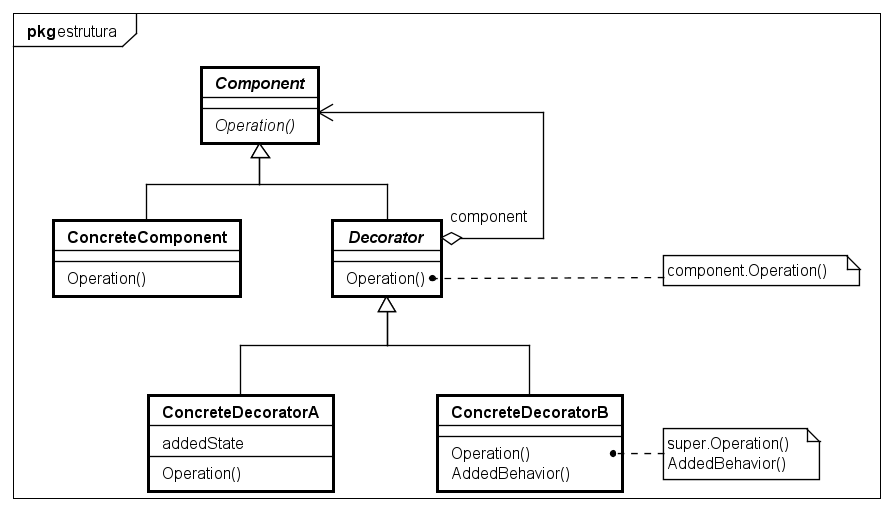
\includegraphics[scale=0.5]{5_padroes-contexto-funcional/5.2_estruturais/5.2.4_decorator/decorator_estrutura.png}
	\end{center}
  \caption*{Fonte: O Autor (2021)}
\end{figure}

\subsection*{Exemplo Orientado a Objetos}

Como exemplo, é apresentado uma ferramenta  
gráfica que permite que diversas funcionalidades, 
como bordas ou barras de rolagem, possam ser adicionadas 
a qualquer componente. Ao invés de usar herança, 
o que exigiria que houvesse uma subclasse para cada 
combinação de funcionalidades e elementos gráficos, 
o padrão \textit{Decorator} é utilizado. Por exemplo, um 
elemento de texto pode ser decorado com uma barra 
de rolagem ou com uma borda. A Figura \ref{decorator_exemplo} 
demonstra o diagrama de classes para esse caso, 
onde uma classe \texttt{TextView} implementa uma interface 
\texttt{VisualComponent}, assim como a classe abstrata \texttt{Decorator}, 
que armazena em seus atributos um objeto do tipo 
\texttt{VisualComponent}. As classes \texttt{ScrollDecorator} e 
\texttt{BorderDecorator} herdam de \texttt{Decorator}, o que faz com que 
elas implementem \texttt{VisualComponent}. Uma das 
possibilidades desse cenário é que um objeto do tipo 
\texttt{ScrollDecorator} armazene um \texttt{BorderDecorator}, que 
por sua vez armazenará um \texttt{TextView}. A operação 
\texttt{Draw} será chamada, em sequência, para cada 
elemento da pilha, resultando no \texttt{TextView} 
com as funcionalidades desejadas. O Código 
\ref{oodecorator} traz a implementação dessa 
abordagem.

\begin{figure}[htb]
	\caption{\label{decorator_exemplo}Exemplo de \textit{Decorator}.}
	\begin{center}
	    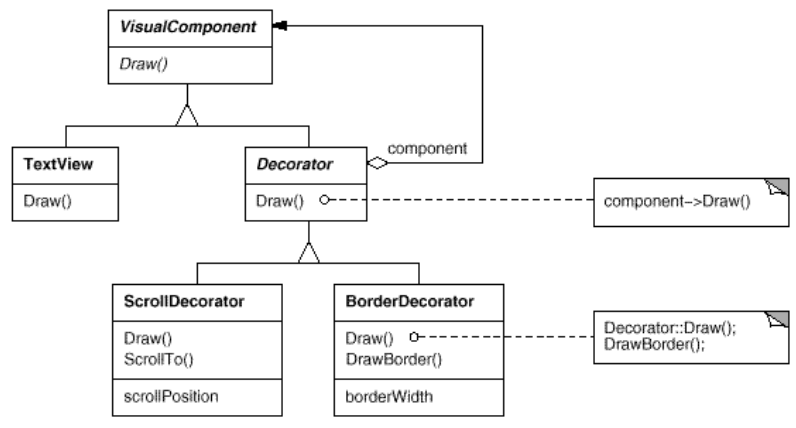
\includegraphics[scale=0.5]{5_padroes-contexto-funcional/5.2_estruturais/5.2.4_decorator/decorator_exemplo.png}
	\end{center}
  \caption*{Fonte: O Autor (2021)}
\end{figure}

\begin{lstlisting}[caption={\textit{Decorator} Orientado a Objetos.},label=oodecorator]

trait VisualComponent {
  def Draw()
}

class TextView extends VisualComponent {
  def Draw(): Unit = {
    //Desenha o componente
  }
}

abstract class Decorator(val component : VisualComponent) extends VisualComponent {
  override def Draw(): Unit = {
    component.Draw()
  }
}

class ScrollDecorator(visualComponent: VisualComponent)
  extends Decorator(visualComponent) {

  var ScrollPosition : Int = 0

  override def Draw() : Unit = {
    //Desenha Scroll
    super.Draw()
  }
}

class BorderDecorator(visualComponent: VisualComponent)
  extends Decorator(visualComponent){

  var BorderWidth : Int = 0

  override def Draw(): Unit = {
    //Desenha Border
    super.Draw()
  }
}

\end{lstlisting}
\legend{Fonte: O Autor (2021)}

\subsection*{Contexto Funcional}

Para que o \textit{Decorator} possa ser usado no contexto 
funcional para estender operações, as funções 
decoradoras devem receber como parâmetro uma função 
que possua a mesma assinatura da função decorada. 
Elas também devem retornar uma função que receba 
como parâmetro os valores de entrada para a 
função decorada. Internamente, as funções decoradoras 
chamam a função recebida como parâmetro e realizam 
qualquer operação adicional necessária. 

Com essa implementação, a função resultante de uma 
função decoradora possui a mesma assinatura da função 
decorada, fazendo com que a aplicação não precise adaptar 
os parâmetros ao utilizá-la. Isso também permite 
encadear as funções decoradoras, trazendo uma estrutura de 
pilha, semelhante à implementação orientada a objetos.

O Código \ref{fpdecorator} demonstra o exemplo anterior, onde 
a função \texttt{DrawTextView}, na linha 2, recebe como parâmetro uma 
\textit{string} e cria um \textit{text view} que a exibe. As funções 
\texttt{DrawTextScroll}, na linha 4, e \texttt{DrawBorder}, na linha 11, decoram 
a função \texttt{DrawTextView}, exibindo também uma barra de \textit{scroll} 
e bordas para o componente. Por fim, o valor \texttt{DecoratedDraw}, na 
linha 18, encadeia as três funções, criando uma nova função 
com a mesma assinatura de \texttt{DrawTextView} com as funcionalidades 
adicionais.

\begin{lstlisting}[caption={\textit{Decorator} Funcional.},label=fpdecorator]
    
def DrawTextView(text : String) : Unit = println(text)

def DrawTextScroll(position : Int, Draw : (String) => Unit) : (String) => Unit = {
  (text : String) => {
    println("Scroll at " + position)
    Draw(text)
  }
}

def DrawBorder(width : Int, Draw : (String) => Unit) : (String) => Unit = {
  (text : String) => {
  println("Border of width " + width)
  Draw(text)
  }
}

val DecoratedDraw : (String) => Unit =
  DrawBorder(3,
    DrawTextScroll(5,
      Draw))
    
\end{lstlisting}
\legend{Fonte: O Autor (2021)}